\documentclass[11pt,a4paper]{article}
\usepackage[margin=1in]{geometry}
\usepackage{amsmath}
\usepackage{booktabs}
\usepackage{graphicx}
\usepackage{xcolor}
\usepackage[hidelinks]{hyperref}
\graphicspath{{../figs/}}

\newcommand{\Szero}{\ensuremath{\Sigma^0}}
\newcommand{\Lam}{\ensuremath{\Lambda}}
\newcommand{\numubar}{\ensuremath{\bar\nu_\mu}}
\newcommand{\FoM}{\ensuremath{S/\sqrt{S+B}}}
\newcommand{\ten}[1]{\ensuremath{\times10^{#1}}}

\title{\Szero\ Selection for the MicroBooNE Hyperon Analysis\\
\large PeLEE ntuples, RHC --- selection, reconstruction, and BDT}
\author{J.\ Nowak}
\date{\today}

\begin{document}
\maketitle

\begin{abstract}
This note documents the event selection for the \numubar\ charged-current
\Szero\ ($\Szero\!\to\!\Lam\gamma$, $\Lam\!\to\!p\pi^-$) search in MicroBooNE,
built on standard PeLEE ntuples in reverse-horn-current (RHC) running.
The selection identifies the muon, proton, pion and photon candidates,
reconstructs the \Lam\ and \Szero\ invariant masses, and applies a
gradient-boosted decision tree (BDT) as the final discriminant, evaluated with
two-fold cross-validation. The final selection keeps $502$ raw signal events
($12.1\%$ of the true \Szero\ in the fiducial volume) at a significance \FoM\ of
$0.0537$, a $19.5\%$ improvement over the cut-based selection. The surviving
background is dominated by resonant and deep-inelastic neutrino interactions
with $\pi^0$ production.
\end{abstract}

\section{Signal and samples}
The signal is the production of a \Szero\ hyperon in \numubar\ CC interactions,
\[
  \numubar + \mathrm{Ar} \;\to\; \mu^+ + \Szero + X,\qquad
  \Szero \to \Lam\,\gamma,\qquad \Lam \to p\,\pi^-,
\]
giving a final state of a $\mu^+$, a displaced $p\pi^-$ vertex from the \Lam\
decay, and a photon from the \Szero. Signal events are flagged at truth level by
$\mathrm{nu\_pdg}=-14$, $\mathrm{ccnc}=0$ and a \Szero\ ($\mathrm{pdg}=3212$) in
the final-state list, with the true vertex inside the fiducial volume.

\begin{table}[h]
\centering
\caption{Samples and POT normalisation. All samples are scaled to the full RHC
data exposure. The background uses all five RHC overlay runs.}
\label{tab:samples}
\begin{tabular}{llrr}
\toprule
Sample & Source & Generated POT & Scale factor \\
\midrule
Signal (\Szero) & NuWro hyperon, NoCR & $2.1764\ten{23}$ & $0.0053$ \\
Other hyperons  & NuWro hyperon, NoCR & $2.1764\ten{23}$ & $0.0053$ \\
Background       & GENIE RHC overlay (Run\,1+2+4a+4b+4c) & $9.9448\ten{21}$ & $0.1159$ \\
Dirt            & GENIE RHC dirt (Run\,1) & $4.2127\ten{20}$ & $2.7360$ \\
\midrule
\multicolumn{2}{l}{Target data exposure} & $1.1526\ten{21}$ & \\
\bottomrule
\end{tabular}
\end{table}

\section{Candidate reconstruction}
Particle-flow objects (PFPs) are split into tracks ($\mathrm{trk\_score}>0.5$)
and showers. The candidates are chosen as:
\begin{itemize}
  \item \textbf{Muon}: the longest track with $\mathrm{trk\_score}>0.8$,
        distance to vertex $<20$~cm, length $>10$~cm, and LLR PID $>0.7$.
  \item \textbf{Proton / pion (joint assignment)}: among the remaining tracks a
        combined PID discriminant is formed,
        \[ D = \mathrm{LLR}/0.591 + (\chi^2_{p}-\chi^2_{\pi})/124.5, \]
        (high $D$ = pion-like, low = proton-like); the proton is the track with
        $\min D$ and the pion the remaining track with $\max D$. This combination
        separates true protons from true pions with AUC $0.873$, versus $0.838$
        for $\chi^2_{p}$ alone and $0.852$ for the LLR alone (the standardisation
        scales are taken from truth-matched tracks). The LLR is always defined, so
        no fallback is needed; the $\chi^2$ term is dropped per track where
        undefined. This reduces proton contamination of the pion candidate from
        $35\%$ (original ``max-LLR'' pion) to $28\%$ (true-pion fraction $31\%$),
        and raises the proton-candidate purity to $58\%$.
  \item \textbf{Photon}: the shower closest to the vertex (shower\,1); a second
        shower (shower\,2) is also retained for $\pi^0$ rejection.
\end{itemize}

\paragraph{\Lam\ and \Szero\ invariant masses.}
The proton momentum is obtained from its range-based kinetic energy (proton
hypothesis), the pion momentum from the range momentum (MIP hypothesis), and
directions from \texttt{trk\_dir}. The photon four-vector uses the
\emph{per-PFP} shower energy \texttt{shr\_energy\_y\_v} (which, unlike the scalar
shower-energy branch, is populated) and the unit direction
\texttt{shr\_px/py/pz\_v}:
\[
  m_\Lam = \sqrt{(E_p+E_\pi)^2-|\vec p_p+\vec p_\pi|^2},\qquad
  m_\Szero = \sqrt{(E_\Lam+E_\gamma)^2-|\vec p_\Lam+\vec p_\gamma|^2}.
\]
The reconstructed signal \Lam\ peaks at $1.111$~GeV (PDG $1.1157$~GeV);
the \Szero\ mean lands on the PDG value $1.1926$~GeV.

\section{Selection chain}
The cumulative cut chain (and the surviving yields) is given in
Table~\ref{tab:cutflow}. The first eight stages are simple requirements; the
ninth is the BDT. The old hard discriminating cuts (proton--muon distance,
photon shower size, \Lam-mass window) were removed --- they are now BDT inputs,
so their power is retained and combined optimally.

\begin{table}[h]
\centering
\caption{Cut flow. ``Raw \Szero'' is the unweighted signal count; efficiency is
relative to the true \Szero\ in the fiducial volume; $S$, $B$ are POT-weighted
signal and total background; \FoM\ is the significance.}
\label{tab:cutflow}
\begin{tabular}{lrrrrrr}
\toprule
Cut & Raw \Szero & Eff.\,[\%] & $S$ & $B$ & Pur.\,[\%] & \FoM \\
\midrule
AllEvents       & 4148 & 100.00 & 21.967 & 691965.9 & 0.003 & 0.0264 \\
FiducialV       & 3375 & 81.36  & 17.874 & 121860.4 & 0.015 & 0.0512 \\
CosmicVeto      & 2969 & 71.58  & 15.724 & 74052.9  & 0.021 & 0.0578 \\
NShowers        & 2333 & 56.24  & 12.355 & 33188.5  & 0.037 & 0.0678 \\
MuonCandidate   & 2097 & 50.55  & 11.106 & 22927.4  & 0.048 & 0.0733 \\
ProtonCandidate & 1449 & 34.93  & 7.674  & 18725.0  & 0.041 & 0.0561 \\
PionCandidate   & 682  & 16.44  & 3.612  & 10571.1  & 0.034 & 0.0351 \\
NTracksCut      & 650  & 15.67  & 3.442  & 8261.8   & 0.042 & 0.0379 \\
\textbf{BDTG}   & \textbf{502} & \textbf{12.10} & \textbf{2.659} & \textbf{2452.3} & \textbf{0.108} & \textbf{0.0537} \\
\bottomrule
\end{tabular}
\end{table}

\noindent The discrete cuts are: fiducial volume (vertex inside the TPC with the
dead $z$ region $675.1$--$775.1$~cm removed); cosmic veto
$\mathrm{topological\_score}>0.20$; shower multiplicity $0<n_\mathrm{shr}<4$;
muon/proton/pion candidate existence; track multiplicity $n_\mathrm{trk}<5$.

\section{BDT discriminant}
A gradient-boosted BDT (TMVA, \texttt{BoostType=Grad}, $N_\mathrm{trees}=600$,
\texttt{MaxDepth}=3, \texttt{Shrinkage}=0.06, \texttt{MinNodeSize}=3\%,
bagged fraction 0.5) is trained at the NTracksCut preselection on
$49$ candidate-level variables --- track PID/length/score/hits, inter-candidate
distances and opening angles, the \Lam\ and \Szero\ masses, shower energy/size,
$\Lam/\gamma$ vertex-pointing variables, and $\pi^0$ variables (di-photon mass,
opening angle, second-shower energy).

\paragraph{Two-fold cross-validation.}
To avoid applying the BDT to its own training events, two folds are trained ---
fold A on even event numbers, fold B on odd --- and each event is scored by the
fold that did \emph{not} train on it. Per-fold ROC integrals are $0.822$ and
$0.809$. The most important variables are the engineered ones: $m_\Szero$,
proton track score, $\gamma$-pointing angle, $m_\Lam$, pion PID, and the
soft-photon shower size; the $\pi^0$ di-photon mass also contributes.

\paragraph{Operating point.}
The threshold $\mathrm{BDTG}>-0.90$ is chosen signal-first: it keeps $502$ raw
signal events (above the cut-based $497$) while improving the significance by
$19.5\%$ over the cut-based selection ($\FoM = 0.0537$ vs $0.0449$). The
significance is flat over a broad threshold range and reaches $\approx 0.061$ at
higher purity if more signal can be traded.

\section{Background characterisation}
Table~\ref{tab:bkg} breaks the surviving background down by neutrino interaction
mode. It is dominated by pion-producing resonant (RES) and deep-inelastic (DIS)
events: the $\pi^0\!\to\!\gamma\gamma$ supplies a fake \Szero\ photon and the
charged hadrons fake the proton/pion tracks. Cosmics are only $3\%$ and are
rejected hardest by the BDT.

\begin{table}[h]
\centering
\caption{Surviving background by interaction type (final selection), raw MC
events and POT-scaled yield.}
\label{tab:bkg}
\begin{tabular}{lrrr}
\toprule
Mode & Raw & Scaled & \% of bkg \\
\midrule
Resonant (RES)       & 12549 & 1381.8 & 52.3 \\
Deep inelastic (DIS) & 5576  & 635.3  & 24.0 \\
Quasi-elastic (QE)   & 2543  & 363.8  & 13.8 \\
Meson exch.\ (MEC)   & 1154  & 177.1  & 6.7  \\
Cosmic               & 618   & 74.6   & 2.8  \\
Coherent (COH)       & 71    & 8.9    & 0.3  \\
\midrule
Total                & 22819 & 2643.1 & 100  \\
\bottomrule
\end{tabular}
\end{table}

\paragraph{Candidate purity (background, truth-matched).}
The muon candidate is a true muon $81\%$ of the time; the proton is a true
proton $58\%$; the pion is true $\pi^\pm$ $31\%$ (another proton $28\%$); the
photon shower is a true photon $29\%$ (a proton $18\%$). The signal sample is
cosmic-free by construction (NoCR), and its non-muon truth matching is
unreliable, so only the background purities are quoted.

\section{Control distributions}
Figure~\ref{fig:control} shows the key discriminants at the preselection stage.

\begin{figure}[h]
\centering
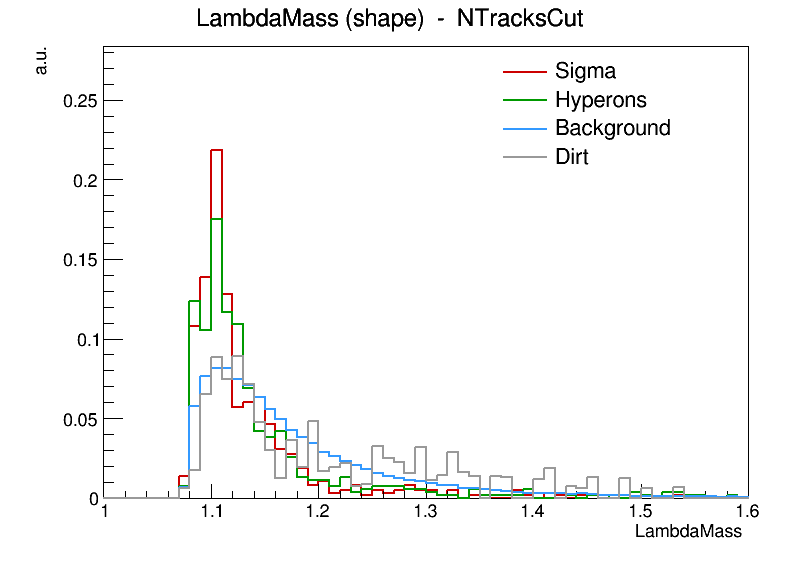
\includegraphics[width=0.45\textwidth]{shape/NTracksCut/LambdaMass.png}
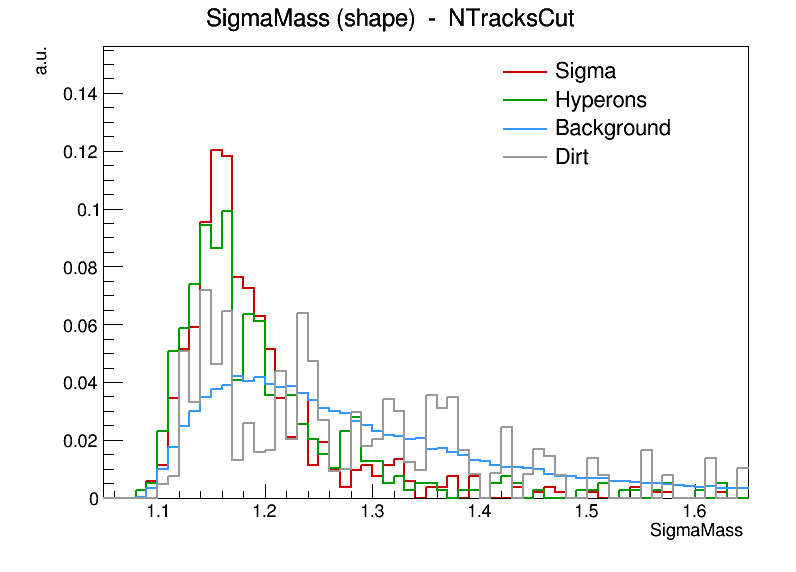
\includegraphics[width=0.45\textwidth]{shape/NTracksCut/SigmaMass.png}\\[2pt]
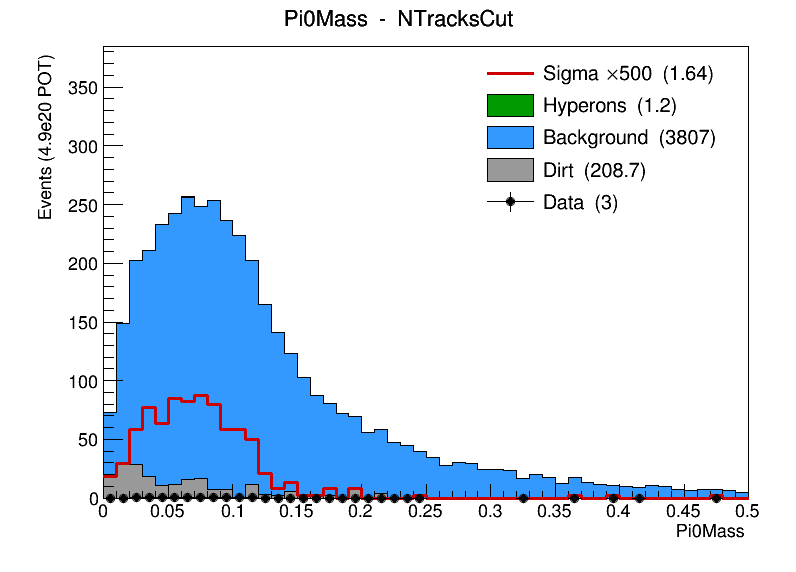
\includegraphics[width=0.45\textwidth]{stack/NTracksCut/Pi0Mass.png}
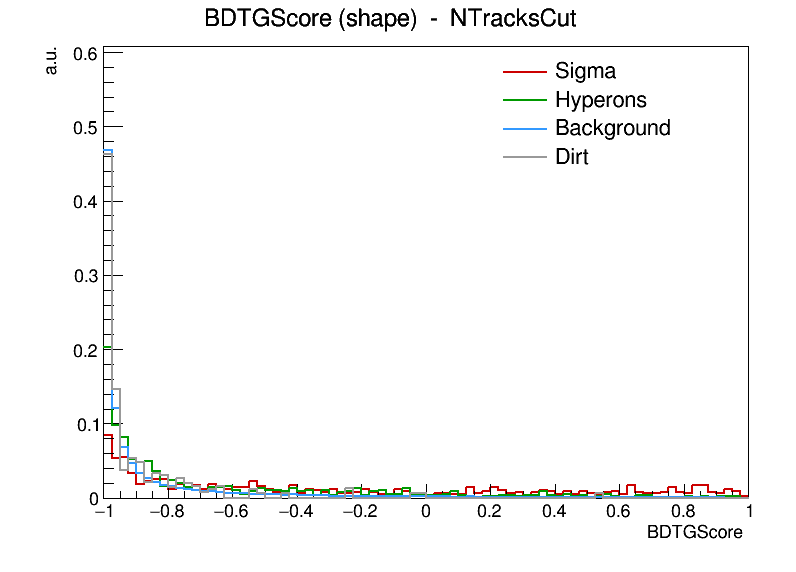
\includegraphics[width=0.45\textwidth]{shape/NTracksCut/BDTGScore.png}
\caption{Preselection-stage distributions: reconstructed \Lam\ mass (top left)
and \Szero\ mass (top right) shapes; $\pi^0$ di-photon mass stack (bottom left);
cross-validated BDT score, signal vs background (bottom right).}
\label{fig:control}
\end{figure}

\section{Summary and limitations}
The selection combines a physics-driven candidate reconstruction
($\Lam\!\to\!p\pi^-$, $\Szero\!\to\!\Lam\gamma$ masses) with a cross-validated
BDT to reach $\FoM=0.0530$ at $12.2\%$ signal efficiency. The analysis is now
\emph{signal-statistics limited}: with $650$ signal events at preselection the
per-fold ROC plateaus at $\approx 0.81$ irrespective of the (much larger)
background sample or additional input variables. The largest remaining lever is
more signal Monte Carlo. Secondary improvements would come from real
shower-energy calibration (to sharpen the \Szero\ mass) and a dedicated $\pi^0$
veto using fully reconstructed di-photon events.

\paragraph{Software.} Selection: \texttt{SigmaSelection.C} (+\texttt{SigmaSelConfig.h},
\texttt{SigmaFV.h}); BDT training: \texttt{TrainBDT.C} (two folds
\texttt{SigmaBDT\_A/}, \texttt{SigmaBDT\_B/}); plotting: \texttt{PlotSigma.C}.

\end{document}
